\documentclass[10pt]{article}
\usepackage[margin=0.9in]{geometry}
\usepackage{booktabs,graphicx,enumitem,xcolor,hyperref}
\setlist{itemsep=1pt,topsep=2pt}
\newcommand{\good}[1]{\textcolor{teal}{#1}}
\newcommand{\bad}[1]{\textcolor{red!70!black}{#1}}
\title{SchNet results: reproducing Fu et al.\ and testing the margin loss}
\author{CS230 project --- results snapshot, \today}
\date{}
\begin{document}
\maketitle
\vspace{-2em}

\section*{Key findings}
\begin{itemize}
  \item \good{Stage A reproduces Fu et al.}\ Force error matches within 5\% on naphthalene and aspirin
        (22.7 vs 22.5 and 36.8 vs 35.6~meV/\AA). Naphthalene \emph{median} time to failure is
        \textbf{18.0~ps}, Fu reports \textbf{18~ps}; ethanol 226 vs 247~ps mean. Salicylic acid is less stable
        than Fu's (3/5 vs 5/5 runs reach 300~ps).
  \item Under Fu's bond rule, the margin loss looks like a big win: mean time to failure
        25~$\to$~131~ps (naphthalene) and 61~$\to$~221~ps (aspirin), with only $\sim$3\% higher force error.
  \item \bad{Most of that gain is not real.} The margin-loss models learned to keep \emph{bonds} intact
        while the molecule distorts in other ways (e.g.\ a hydrogen folded to 1.9~\AA\ from a carbon it is
        not bonded to; reference: 3.4~\AA). The bond rule cannot see this.
  \item With a stricter check that also watches non-bonded atom pairs, the gain shrinks to
        \textbf{about 1.5$\times$ for naphthalene} (25~$\to$~37~ps) and \textbf{none for aspirin} (34~$\to$~38~ps;
        the $\lambda{=}0$ control is also 38~ps). Our evaluation code's own ``combined'' criterion, written before
        these results, agrees.
  \item Structure accuracy (h(r)) is unchanged in the first 10~ps, but gets steadily worse the longer the
        margin-loss naphthalene runs go (0.11~$\to$~0.35).
  \item \textbf{Bottom line:} as currently trained and tuned, the margin loss mostly teaches SchNet to avoid
        the failure \emph{detector}, not to stay physical. It should not yet be claimed as a stability
        improvement. Fix: train and select $\lambda$ with a failure definition that includes non-bonded
        distortions.
\end{itemize}

\section*{What we ran}
\begin{itemize}
  \item \textbf{Data:} Fu et al.'s own MD17 splits (9,500 train / 500 val / 10,000 test), original MD17 at 500~K.
  \item \textbf{Stage A:} SchNet trained with the authors' code and settings (MDsim), 3 seeds for naphthalene
        and aspirin, 1 seed for ethanol and salicylic acid.
  \item \textbf{Stage B (margin loss):} simulate from training frames, collect bond failures, push their energy
        up with the margin loss. $\lambda$ chosen on held-out \emph{tune} frames; 3 seeds.
        $\lambda{=}0$ = same extra training without the margin term (control).
  \item \textbf{Fu-style test:} 5 simulations per model, Nos\'e--Hoover 500~K, 0.5~fs steps, up to 300~ps,
        from 5 fixed test frames. Failure = any bond more than 0.5~\AA\ from its average length.
  \item \textbf{Strict check (ours):} failure = any atom pair (bonded or not) more than 0.5~\AA\ outside the
        range it ever takes in the full MD17 reference trajectory of that molecule. Never triggers on the reference data itself.
  \item \textbf{h(r):} distribution of all interatomic distances vs.\ the reference, computed exactly as in
        Fu et al.'s notebook (lower is better).
\end{itemize}

\section*{1.\ Stage A vs.\ Fu et al.}
\begin{center}
\begin{tabular}{lcccccc}
\toprule
 & \multicolumn{2}{c}{Force error (meV/\AA)} & \multicolumn{2}{c}{Time to failure (ps)} & \multicolumn{2}{c}{h(r) error} \\
\cmidrule(lr){2-3}\cmidrule(lr){4-5}\cmidrule(lr){6-7}
Molecule & Ours & Fu & Ours: mean$\pm$SD (median) & Fu & Ours & Fu \\
\midrule
Naphthalene    & 22.7 & 22.5 & 25 $\pm$ 24 (18.0) & 18 $\pm$ 2 & 0.10 & 0.09 \\
Aspirin        & 36.8 & 35.6 & 61 $\pm$ 78 (20.9) & 26 $\pm$ 23 & 0.06 & 0.36 \\
Ethanol        & 18.4$^*$ & 16.8 & 226 $\pm$ 100 (285) & 247 $\pm$ 106 & 0.16 & 0.21 \\
Salicylic acid & 29.2$^*$ & 26.3 & 188 $\pm$ 154 (300) & 300 $\pm$ 0 & 0.05 & 0.03 \\
\bottomrule
\end{tabular}
\end{center}
{\small Naphthalene/aspirin: 3 models $\times$ 5 simulations, force error on the 10,000 test frames.
Ethanol/salicylic acid: 1 model $\times$ 5 simulations; $^*$force error on the 500 validation frames (test evaluation not run).
Fu: 1 model $\times$ 5 simulations.}

\begin{center}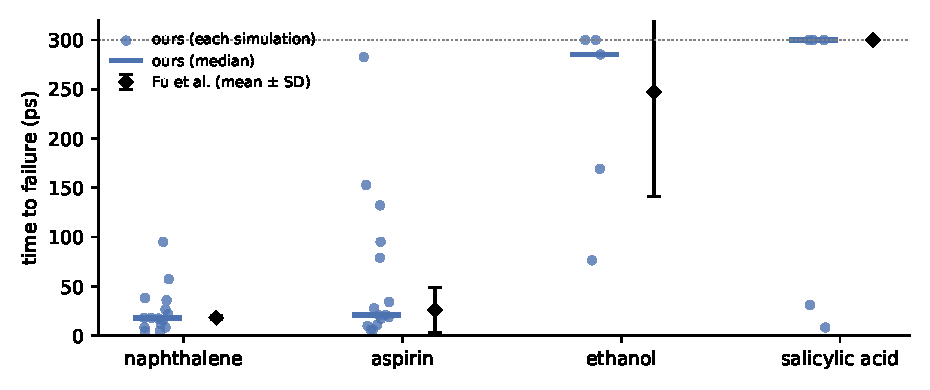
\includegraphics[width=0.72\linewidth]{figures/stageA_vs_fu.pdf}\end{center}
\begin{itemize}
  \item Accuracy matches: within 5\% on naphthalene/aspirin (test), 10--11\% higher on ethanol/salicylic acid (validation). Typical stability matches (medians), but our spread is wider than Fu's.
  \item Ethanol: 2/5 runs reach 300~ps; failures at 76 (temperature guard), 169 and 285~ps. Fu: 247 $\pm$ 106, consistent.
  \item Salicylic acid: 3/5 reach 300~ps, 2 fail early (8 and 31~ps). Fu reports 5/5 at 300~ps, so this is the one
        molecule where our Stage A is visibly \emph{less} stable than Fu's (1 model; may be a seed effect, not checked).
  \item The strict check fires much earlier on ethanol (median 45~ps, 0/5 reach 300~ps), so even our
        ``stable'' ethanol runs leave the reference geometry range. Salicylic acid: strict check changes nothing.
  \item No margin-loss (Stage B) runs for ethanol or salicylic acid: Fu's SchNet is already mostly stable there,
        so they leave little room to show an improvement.
  \item Why the wider spread: (i) we train 3 models, and equally accurate models differ a lot
        (aspirin: 15 vs 126~ps mean); (ii) the simulations are chaotic --- the same run repeated on a GPU
        failed at 12~ps once and survived 30~ps another time.
\end{itemize}

\section*{2.\ Margin loss vs.\ baselines}
\begin{center}
\begin{tabular}{lcccccc}
\toprule
 & \multicolumn{3}{c}{Naphthalene ($\lambda{=}3{\times}10^{-3}$)} & \multicolumn{3}{c}{Aspirin ($\lambda{=}10^{-3}$)} \\
\cmidrule(lr){2-4}\cmidrule(lr){5-7}
 & Stage A & $\lambda{=}0$ & Margin & Stage A & $\lambda{=}0$ & Margin \\
\midrule
Force error (meV/\AA)                 & 22.7 & 22.6 & 23.4 & 36.8 & 36.9 & 37.9 \\
\addlinespace
\multicolumn{7}{l}{\emph{Fu-style simulations (15 per column), time to failure in ps: mean (median)}} \\
Bond rule (Fu)                        & 25 (18) & 23 (20) & \good{131 (68)} & 61 (21) & 48 (49) & \good{221 (300)} \\
Strict check                          & 25 (18) & 22 (20) & 37 (33) & 34 (21) & 38 (41) & 38 (37) \\
Reached 300~ps, bond rule             & 0/15 & 0/15 & 3/15 & 0/15 & 0/15 & 9/15 \\
Reached 300~ps, strict check          & 0/15 & 0/15 & \bad{0/15} & 0/15 & 0/15 & \bad{0/15} \\
\addlinespace
\multicolumn{7}{l}{\emph{h(r) error (lower = closer to the real molecule)}} \\
All stable frames                     & 0.097 & 0.092 & \bad{0.161} & 0.064 & 0.062 & \bad{0.093} \\
First 10~ps only                      & 0.105 & 0.102 & 0.113 & 0.084 & 0.085 & 0.085 \\
\addlinespace
\multicolumn{7}{l}{\emph{Many short simulations (Langevin, 3 seeds $\times$ 256 runs $\times$ 300~ps): fraction that failed}} \\
Bond rule                             & 38\% & 34\% & \good{2.5\%} & 86\% & 87\% & \good{26\%} \\
Combined (bond or collision)          & 38\% & 34\% & 30\% & 94\% & 94\% & \bad{95\%} \\
\bottomrule
\end{tabular}
\end{center}

\begin{center}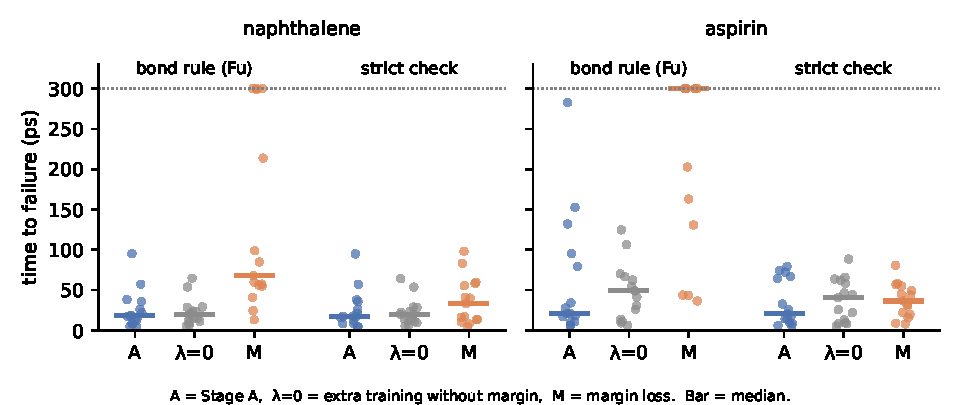
\includegraphics[width=0.85\linewidth]{figures/margin_bond_vs_strict.pdf}\end{center}
\begin{itemize}
  \item With Fu's bond rule (left of each panel) the margin loss (orange) looks far more stable.
        With the strict check (right of each panel) it is only slightly better than the baselines.
  \item $\lambda{=}0$ is no better than Stage A, so whatever gain exists comes from the margin term, not from
        extra training.
\end{itemize}

\section*{3.\ Why the gain disappears: distorted but ``bonded'' states}
\begin{center}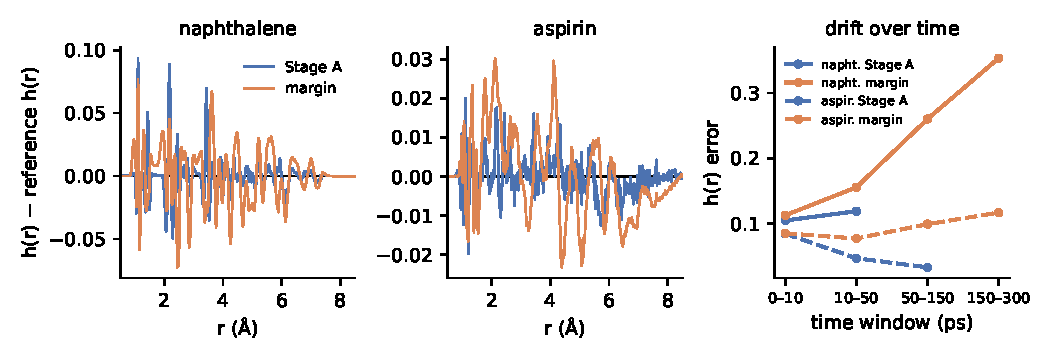
\includegraphics[width=0.95\linewidth]{figures/hr.pdf}\end{center}
\begin{itemize}
  \item Left/middle: difference between each model's h(r) and the reference. The margin model's errors are
        larger, mostly at distances above 3~\AA\ (overall shape of the molecule), not at bond lengths.
  \item Right: h(r) error over time. Early on, margin and Stage A are equally accurate. The longer the
        margin runs go, the worse they get (naphthalene 0.11~$\to$~0.35). A correct model should improve
        with time (more sampling), as Stage A aspirin does.
  \item Example (naphthalene, a run that ``survived'' 300~ps): from $\sim$8~ps on, one hydrogen sits
        1.9~\AA\ from a non-bonded carbon (reference 3.43 $\pm$ 0.07~\AA) and the carbon ring stays bent beyond
        anything in the reference data. Every bond stays within 0.5~\AA, so the bond rule never fires.
  \item Interpretation: the margin loss raises the energy of states \emph{with stretched bonds}, which is what
        it was trained to recognize. The model finds other unphysical states instead.
\end{itemize}

\section*{4.\ How $\lambda$ was chosen, and what changes with the criterion}
\begin{center}
\begin{tabular}{lcc}
\toprule
Selection criterion (tune frames, 2 seeds) & Naphthalene & Aspirin \\
\midrule
Bond rule (used here)        & $\lambda{=}3{\times}10^{-3}$: failures 26\%~$\to$~2\% & $\lambda{=}10^{-3}$: 49\%~$\to$~6\% \\
Combined (repo default)      & best $\lambda$: 26\%~$\to$~19\% (within noise) & no $\lambda$ beats $\lambda{=}0$ (58\%) \\
\bottomrule
\end{tabular}
\end{center}
\begin{itemize}
  \item The bond-only criterion was our choice for these sweeps (to match Fu's metric); the repository default
        is ``combined''. With the default, the sweep would not have reported a large effect.
\end{itemize}

\section*{5.\ Differences from Fu et al.\ and other disclosures}
\begin{itemize}
  \item \textbf{Code fix:} the authors' 2024 code update wraps atoms into a periodic box before each force call.
        SchNet runs without periodic boundaries here, so this tears the molecule apart (forces $\sim$75$\times$
        wrong, failures within 0.05~ps). We use the pre-2024 behavior, under which Fu's SchNet numbers were
        produced, and every run first checks its starting-frame forces against the data (a run with error above
        0.25~eV/\AA\ would abort; none did, typical error 10--25~meV/\AA).
  \item \textbf{Starting frames:} Fu used 5 random test frames (not published); we use 5 fixed ones from our protocol file.
  \item \textbf{Seeds:} we report 3 trained models $\times$ 5 simulations; Fu reports 1 model $\times$ 5 simulations.
  \item \textbf{Hardware:} our GPUs (T4/A10G) differ from Fu's (V100); results are not bit-reproducible.
  \item \textbf{Stage B} starts from a fresh optimizer (the authors' checkpoints do not store optimizer state).
  \item \textbf{Strict check} is our addition, not part of Fu's protocol; we tried margins of 0.3, 0.5 and 1.0~\AA.
        Naphthalene: margin loss 30--40~ps mean vs.\ Stage A 22--25~ps at every margin. Aspirin: the margin-loss median
        stays within a few ps of $\lambda{=}0$ at every margin (31/37/44 vs.\ 27/41/44~ps); only at the loosest
        margin (1.0~\AA) does its mean rise (87 vs.\ 45~ps), driven by a few long runs.
  \item \textbf{Data hygiene:} 5 of 100 saved trajectories contained frames from an interrupted earlier attempt
        (the authors' simulator appends). We keep only the final attempt; reported stability times come from the
        simulation logs and are unaffected. Fixed for future runs.
  \item \textbf{Temperature guard:} one ethanol run stopped at 76~ps because the temperature left the simulator's
        allowed range (upstream rule); we count it as a failure at 76~ps.
  \item \textbf{Langevin test} (``many short simulations'') is our own StABlE-style protocol, not Fu's.
  \item Aspirin h(r): ours 0.06 vs.\ Fu 0.36 $\pm$ 0.57. We have not investigated the difference.
\end{itemize}

\section*{Next steps}
\begin{itemize}
  \item Retrain Stage B so that ``failure'' includes non-bonded distortions (same rule as the strict check),
        and select $\lambda$ with the combined criterion. Then re-run this exact evaluation.
  \item Report the strict check and h(r) alongside Fu's bond rule for every model in the paper.
  \item Repeat for GemNet-T (partner's runs) once Stage A finishes.
\end{itemize}
\end{document}
